\chapter{Results and Discussion}

All results in this chapter are for the lossless problem; losses are treated in Chapter~7. The numbers are produced by the scripts listed in Table~\ref{tab:modules} and stored in the \texttt{results/} folder of the repository.

\section{Hybrid QAOA dispatch}
Figure~\ref{fig:dispatch} shows the hybrid QAOA dispatch for the 12 periods, and Table~\ref{tab:hybrid} compares it with the SLSQP optimum. The cheaper units G2 and G3 carry most of the load, and G1 stays at its 50~MW minimum in periods 2--6, as in the classical solution.

\begin{figure}[H]
\centering
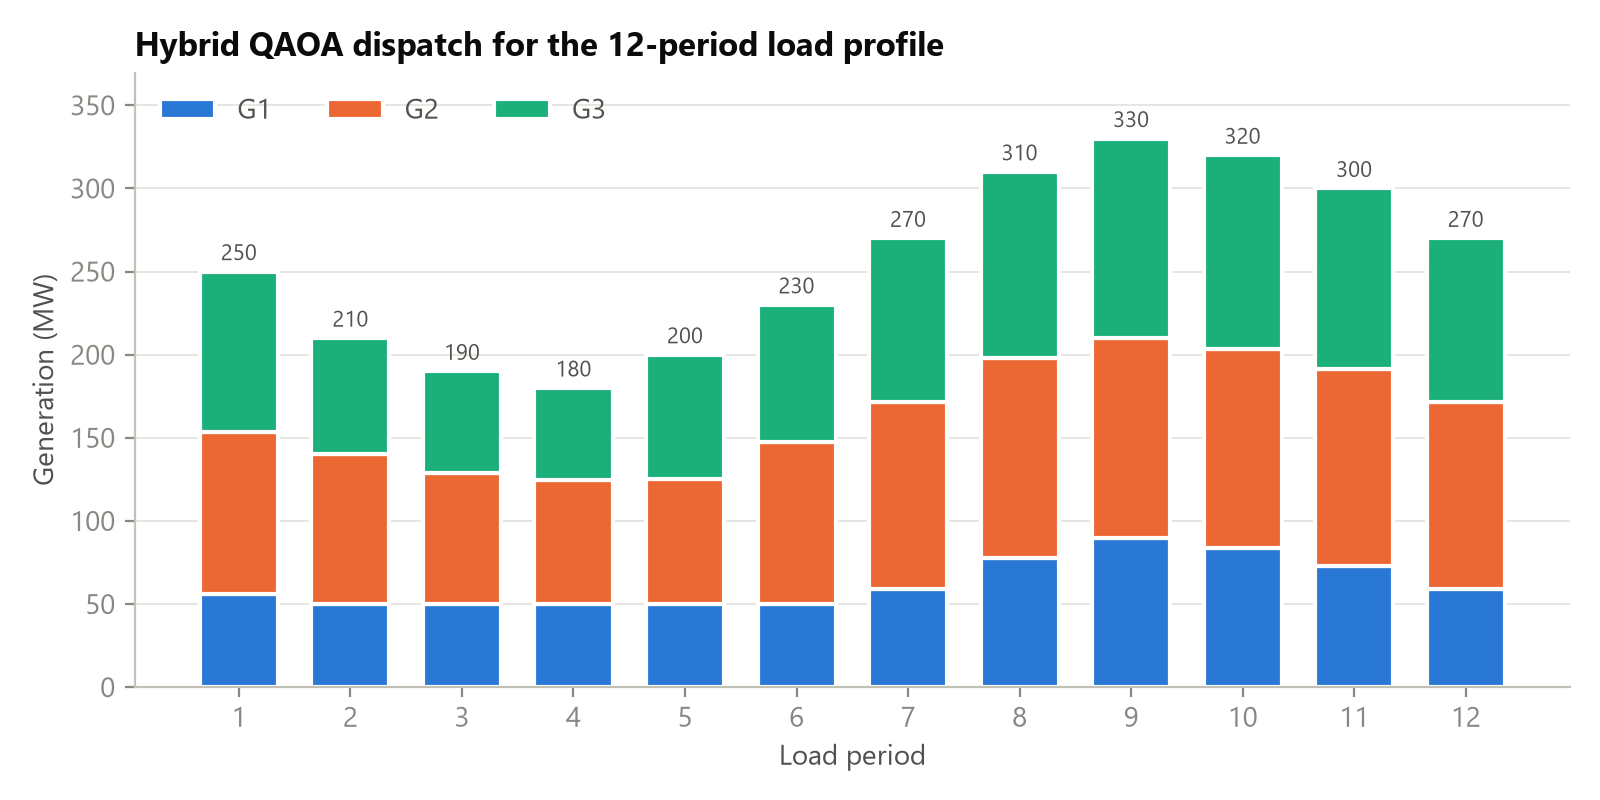
\includegraphics[width=0.92\textwidth]{dispatch_by_period}
\caption{Hybrid QAOA dispatch (12 qubits, $p = 4$, 4096 shots, refinement of the best five bitstrings). Numbers above the bars are the demand in MW.}
\label{fig:dispatch}
\end{figure}

\begin{table}[H]
\centering
\caption{Hybrid QAOA dispatch compared with SLSQP. ``Hits'' is the number of the 4096 shots that returned the exact QUBO optimum.}
\label{tab:hybrid}
\small
\begin{tabular}{ccccrrrc}
\toprule
Period & G1 & G2 & G3 & Hybrid cost & SLSQP cost & Gap (\%) & Hits\\
 & (MW) & (MW) & (MW) & (\$/h) & (\$/h) & & \\
\midrule
1 & 55.89 & 97.50 & 96.61 & 3529.65 & 3528.83 & 0.023 & 1\\
2 & 50.00 & 90.00 & 70.00 & 3046.47 & 3046.41 & 0.002 & 13\\
3 & 50.00 & 78.98 & 61.02 & 2810.05 & 2810.05 & 0.000 & 18\\
4 & 50.00 & 74.44 & 55.56 & 2693.08 & 2693.08 & 0.000 & 34\\
5 & 50.00 & 75.00 & 75.00 & 2929.01 & 2927.83 & 0.040 & 18\\
6 & 50.00 & 97.17 & 82.83 & 3286.01 & 3286.01 & 0.000 & 5\\
7 & 58.80 & 112.50 & 98.70 & 3774.05 & 3774.02 & 0.001 & 4\\
8 & 77.70 & 120.00 & 112.30 & 4269.93 & 4269.91 & 0.000 & 5\\
9 & 90.00 & 120.00 & 120.00 & 4521.12 & 4520.62 & 0.011 & 3\\
10 & 83.52 & 120.00 & 116.48 & 4395.21 & 4395.04 & 0.004 & 12\\
11 & 72.64 & 118.69 & 108.66 & 4145.25 & 4145.25 & 0.000 & 7\\
12 & 58.80 & 112.50 & 98.70 & 3774.05 & 3774.02 & 0.001 & 4\\
\midrule
Total & & & & 43173.88 & 43171.05 & 0.007 & \\
\bottomrule
\end{tabular}
\end{table}

The QUBO optimum was among the measured bitstrings in all 12 periods. After refinement every dispatch meets the demand exactly, and the largest gap is 0.040\,\% (period 5, \$1.18/h). Over the day the hybrid dispatch costs \$2.83 more than the optimum.

The remaining gap is not caused by QAOA. Exhaustive search over all 4096 bitstrings followed by the same refinement gives exactly the same costs (Section~\ref{sec:compare}). It comes from the refinement box: in a few periods the continuous optimum lies more than one grid step from the best grid points. In period 5, for example, the QUBO optimum is (60, 67.5, 72)~MW, while the SLSQP optimum is (50, 83.5, 66.5)~MW; G2 can move only up to 75~MW inside the box, so the refined dispatch stops at (50, 75, 75)~MW.

\section{Cost accuracy and power balance}
Figure~\ref{fig:gap} shows the cost difference of the raw QAOA grid point and of the hybrid dispatch for each period. Some raw grid points appear cheaper than SLSQP; these supply 0.5~MW less than the demand (Figure~\ref{fig:mismatch}) and are not feasible. Refinement removes the mismatch in every period.

\begin{figure}[H]
\centering
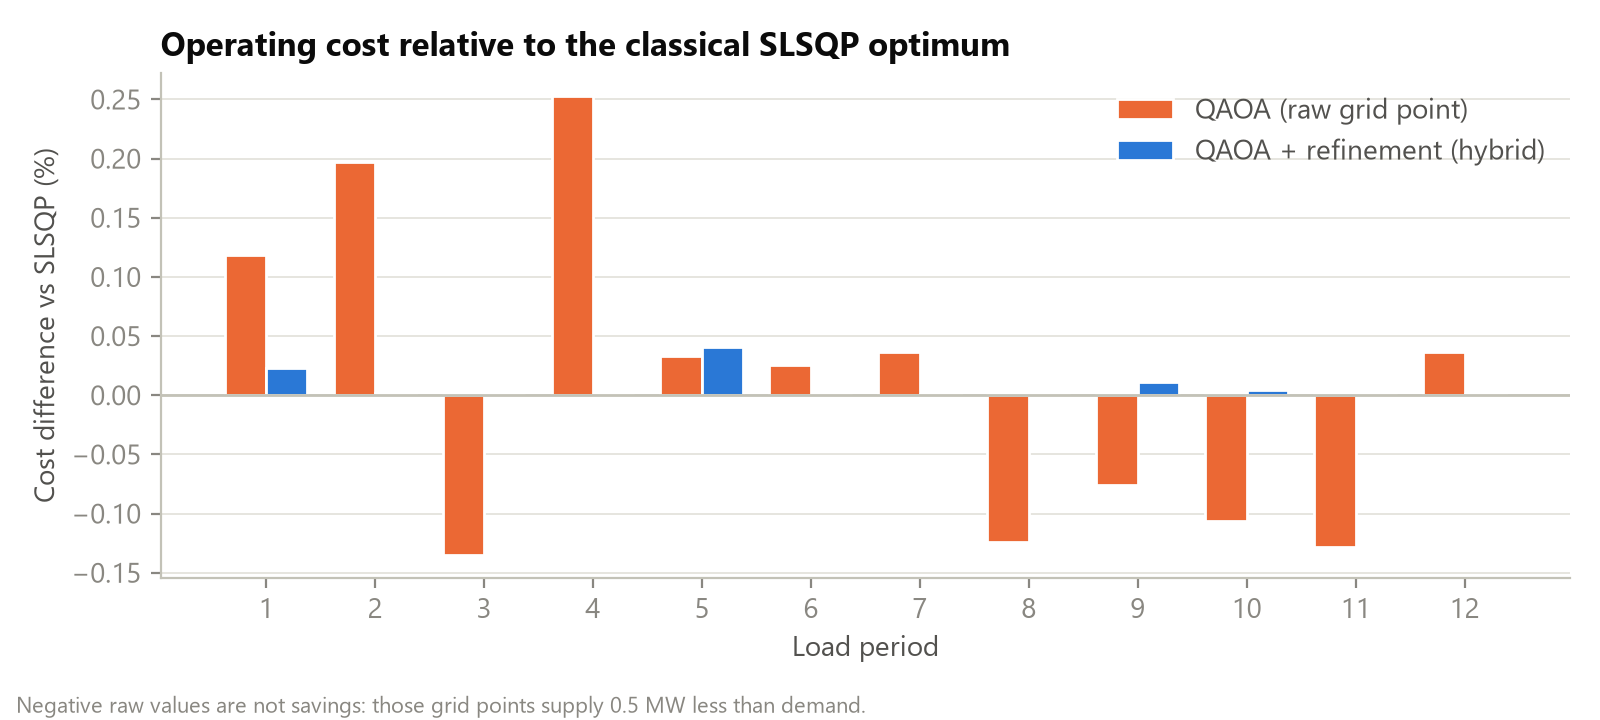
\includegraphics[width=0.92\textwidth]{cost_gap}
\caption{Cost difference relative to SLSQP: raw QAOA grid point and hybrid dispatch.}
\label{fig:gap}
\end{figure}

\begin{figure}[H]
\centering
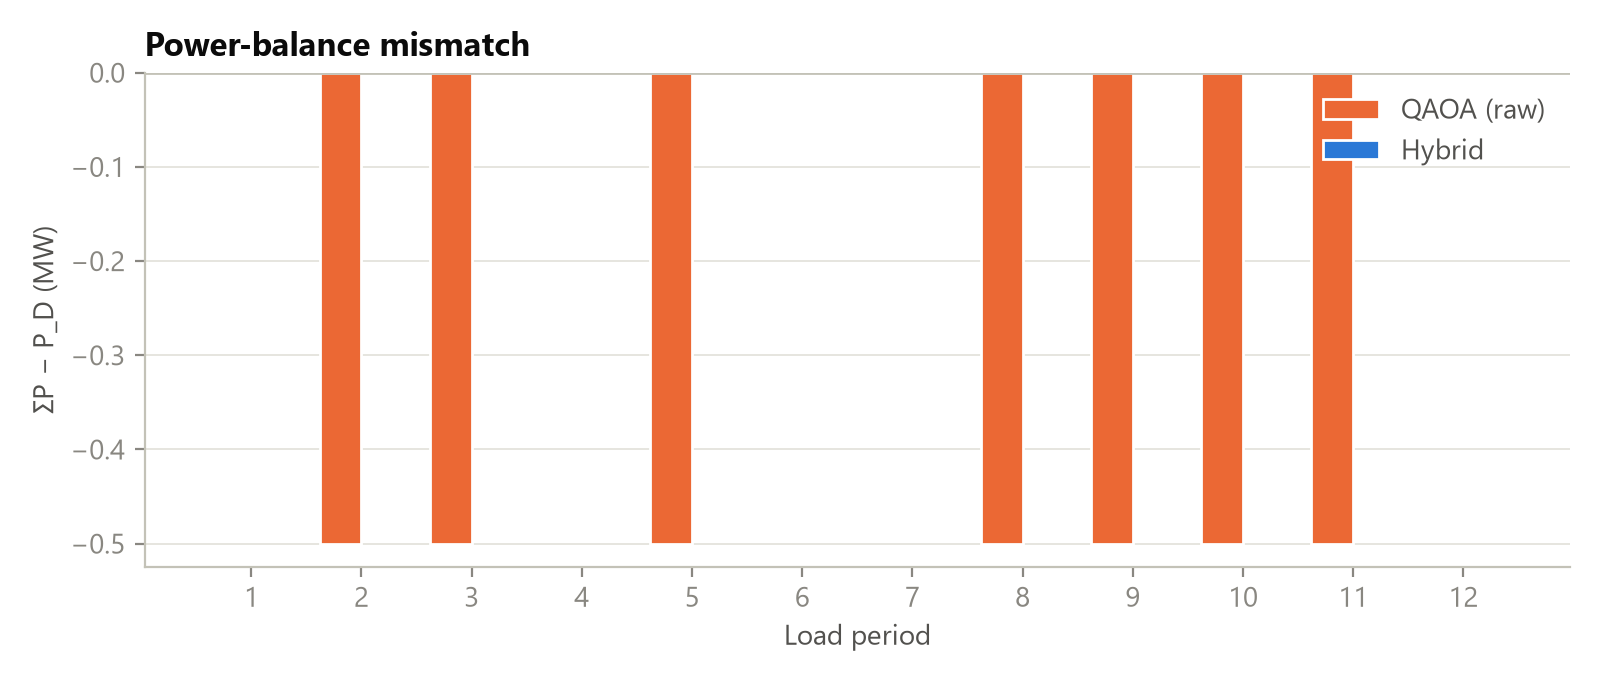
\includegraphics[width=0.92\textwidth]{mismatch}
\caption{Power-balance mismatch $\sum P_i - \PD$ before and after refinement.}
\label{fig:mismatch}
\end{figure}

\section{Effect of circuit depth}
Table~\ref{tab:depth} and Figure~\ref{fig:amp} show how the trained circuit concentrates probability as the depth increases. The amplification of the optimal bitstring rises from 4.6 at $p = 1$ to 10.2 at $p = 4$ on average, and up to 31 in period 4. At $p = 4$, 20.4\,\% of measurements are near-optimal, compared with 3.1\,\% for uniform random sampling (Figure~\ref{fig:pgood}).

\begin{table}[H]
\centering
\caption{QAOA performance against depth (mean over 12 periods; exact statevector).}
\label{tab:depth}
\begin{tabular}{ccccc}
\toprule
$p$ & Amplification & Amplification & Near-optimal & Training\\
 & (mean) & (max) & probability & time (s)\\
\midrule
1 & 4.58 & 15.1 & 10.4\,\% & 3.5\\
2 & 6.76 & 21.3 & 13.9\,\% & 4.0\\
3 & 8.33 & 25.5 & 16.8\,\% & 6.3\\
4 & 10.18 & 31.0 & 20.4\,\% & 8.2\\
\midrule
Random & 1 & 1 & 3.1\,\% & --\\
\bottomrule
\end{tabular}
\end{table}

\begin{figure}[H]
\centering
\begin{minipage}{0.49\textwidth}\centering
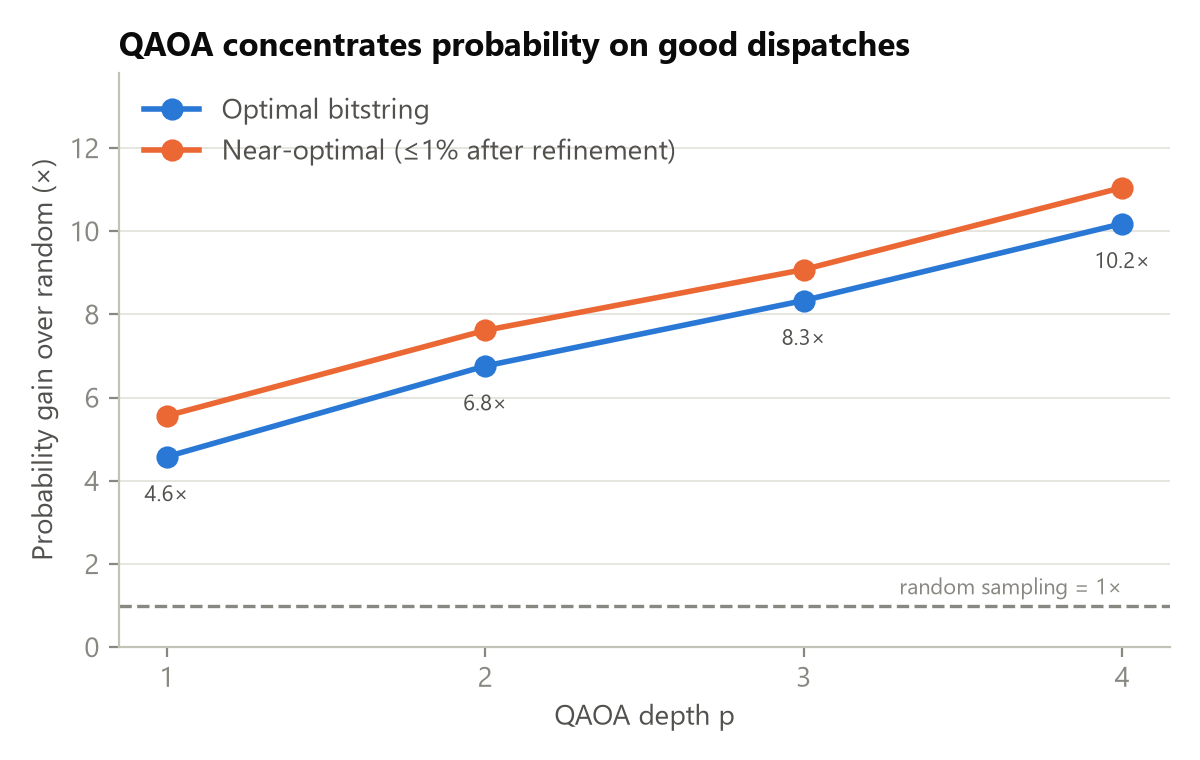
\includegraphics[width=\textwidth]{amplification_vs_depth}
\caption{Probability gain over random sampling against depth.}
\label{fig:amp}
\end{minipage}\hfill
\begin{minipage}{0.49\textwidth}\centering
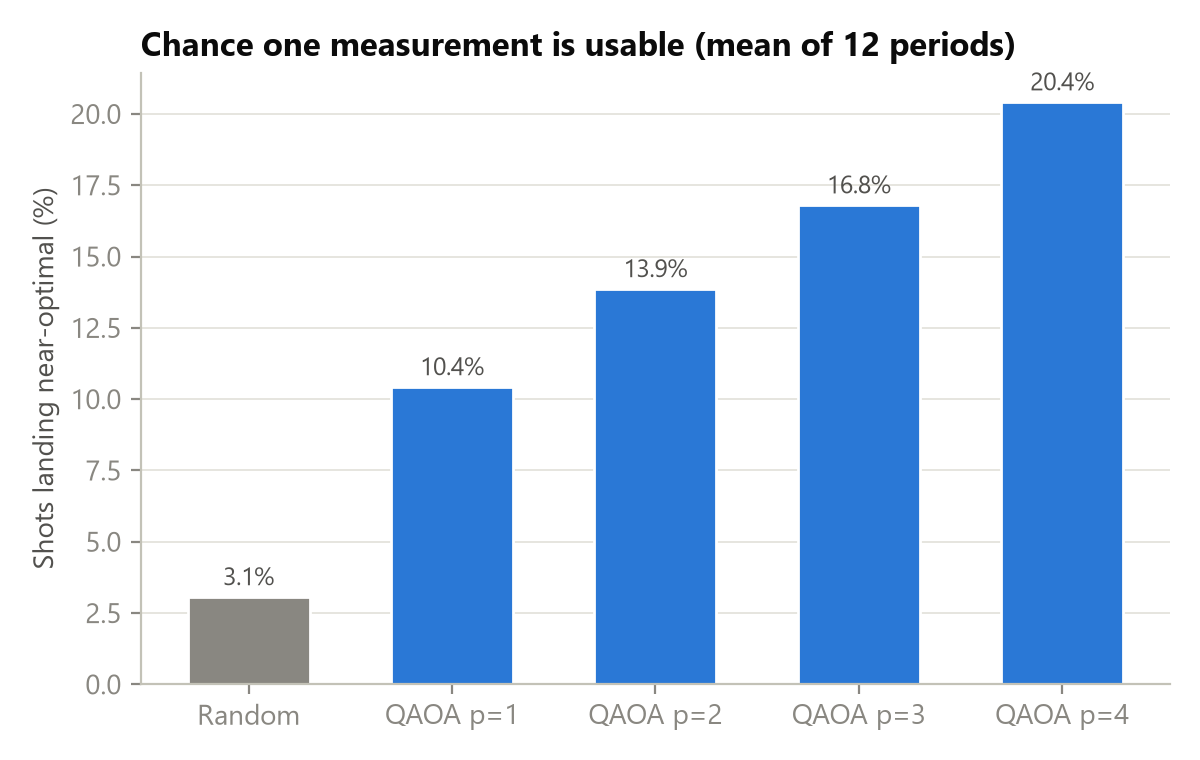
\includegraphics[width=\textwidth]{p_good}
\caption{Chance that one measurement is near-optimal.}
\label{fig:pgood}
\end{minipage}
\end{figure}

The amplification varies strongly between periods: it is highest in periods 2--5 (13.6--31.0 at $p = 4$) and lowest in period 6 (2.4). Figure~\ref{fig:conv} shows the CVaR training curves for period 1 on a logarithmic scale. The $p = 1$ curve (best of eight random starts) begins far from the optimum; the deeper circuits begin from the INTERP extension of the previous optimum, about ten times closer. Depth $p = 4$ reaches the lowest CVaR. In this period $p = 3$ finishes slightly above $p = 2$: COBYLA is a local optimiser, and a single INTERP start does not guarantee monotone improvement. Depths 3 and 4 also use the full 400-iteration budget, so their training time could be reduced with a looser tolerance.

\begin{figure}[H]
\centering
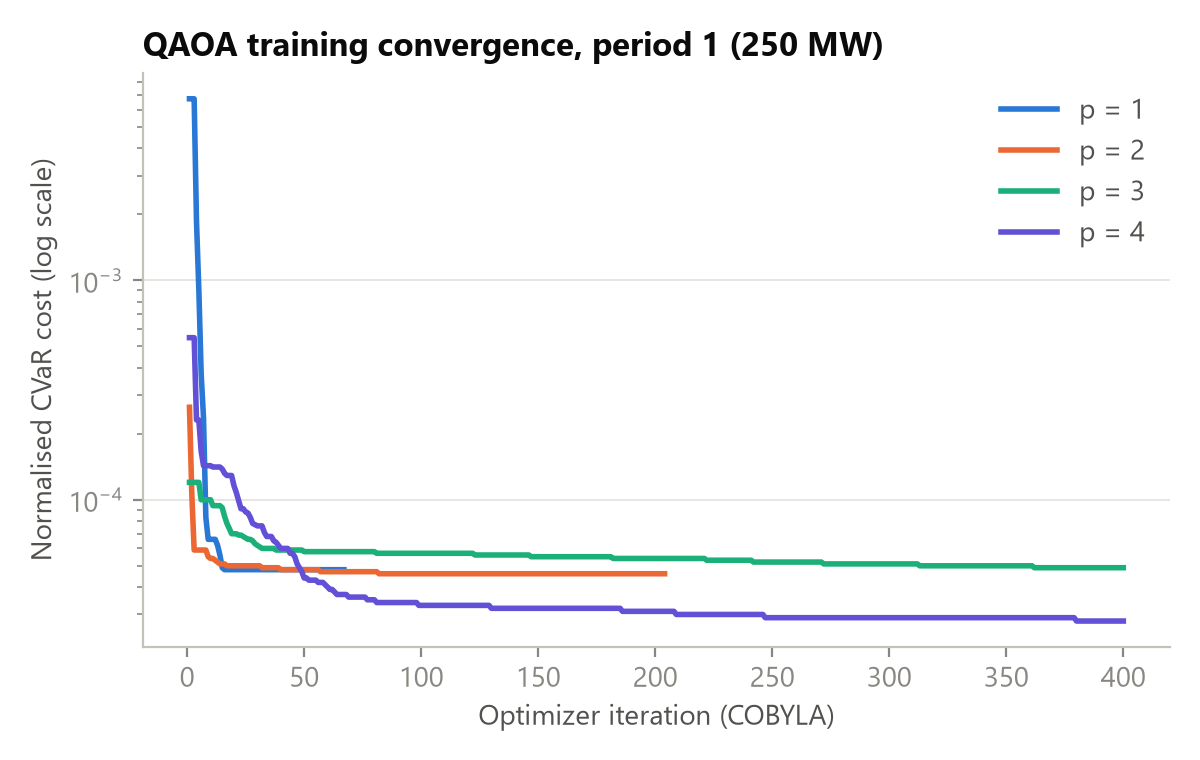
\includegraphics[width=0.7\textwidth]{convergence}
\caption{CVaR training convergence for period 1 (250 MW) at each depth.}
\label{fig:conv}
\end{figure}

\section{Comparison with standard algorithms}
\label{sec:compare}
Table~\ref{tab:compare} compares hybrid QAOA with standard methods over all 12 periods. Every stochastic method was run with 20 random seeds per period (240 runs). Methods that work on the QUBO (exhaustive search, SA and QAOA) all evaluate 4096 bitstrings and refine their five lowest-energy candidates in exactly the same way, so they differ only in how they search the binary space. PSO and GA work on the continuous outputs with a similar budget (3030 evaluations).

\begin{table}[H]
\centering
\caption{Comparison with standard algorithms (12 periods; 20 seeds each for stochastic methods). Success: within 0.1\,\% of SLSQP and $|\text{mismatch}| \le 0.01$~MW.}
\label{tab:compare}
\small
\begin{tabular}{llrrrr}
\toprule
Method & Space & Mean gap & Worst gap & Success & Time/period\\
\midrule
SLSQP (reference) & continuous & 0 & 0 & 100\,\% & 1.3 ms\\
$\lambda$-iteration & continuous & 0 & 0 & 100\,\% & 0.5 ms\\
PSO, dep.\ unit \cite{gaing2003} & continuous & 0.0000\,\% & 0.0003\,\% & 100\,\% & 13 ms\\
GA, dep.\ unit & continuous & 0.0000\,\% & 0.0001\,\% & 100\,\% & 80 ms\\
PSO, penalty & continuous & 0.645\,\% & 2.190\,\% & 13.8\,\% & 10 ms\\
GA, penalty & continuous & 0.763\,\% & 3.011\,\% & 7.5\,\% & 81 ms\\
Exhaustive + refine & 12-bit QUBO & 0.007\,\% & 0.040\,\% & 100\,\% & 10 ms\\
SA + refine & 12-bit QUBO & 0.029\,\% & 0.437\,\% & 92.5\,\% & 71 ms\\
\textbf{QAOA + refine} & 12-bit QUBO & \textbf{0.007\,\%} & \textbf{0.040\,\%} & \textbf{100\,\%} & 0.28 s$^\dagger$\\
\bottomrule
\multicolumn{6}{l}{\footnotesize $^\dagger$ Sampling on a laptop simulator, after about 22~s of training per period.}
\end{tabular}
\end{table}

\begin{figure}[H]
\centering
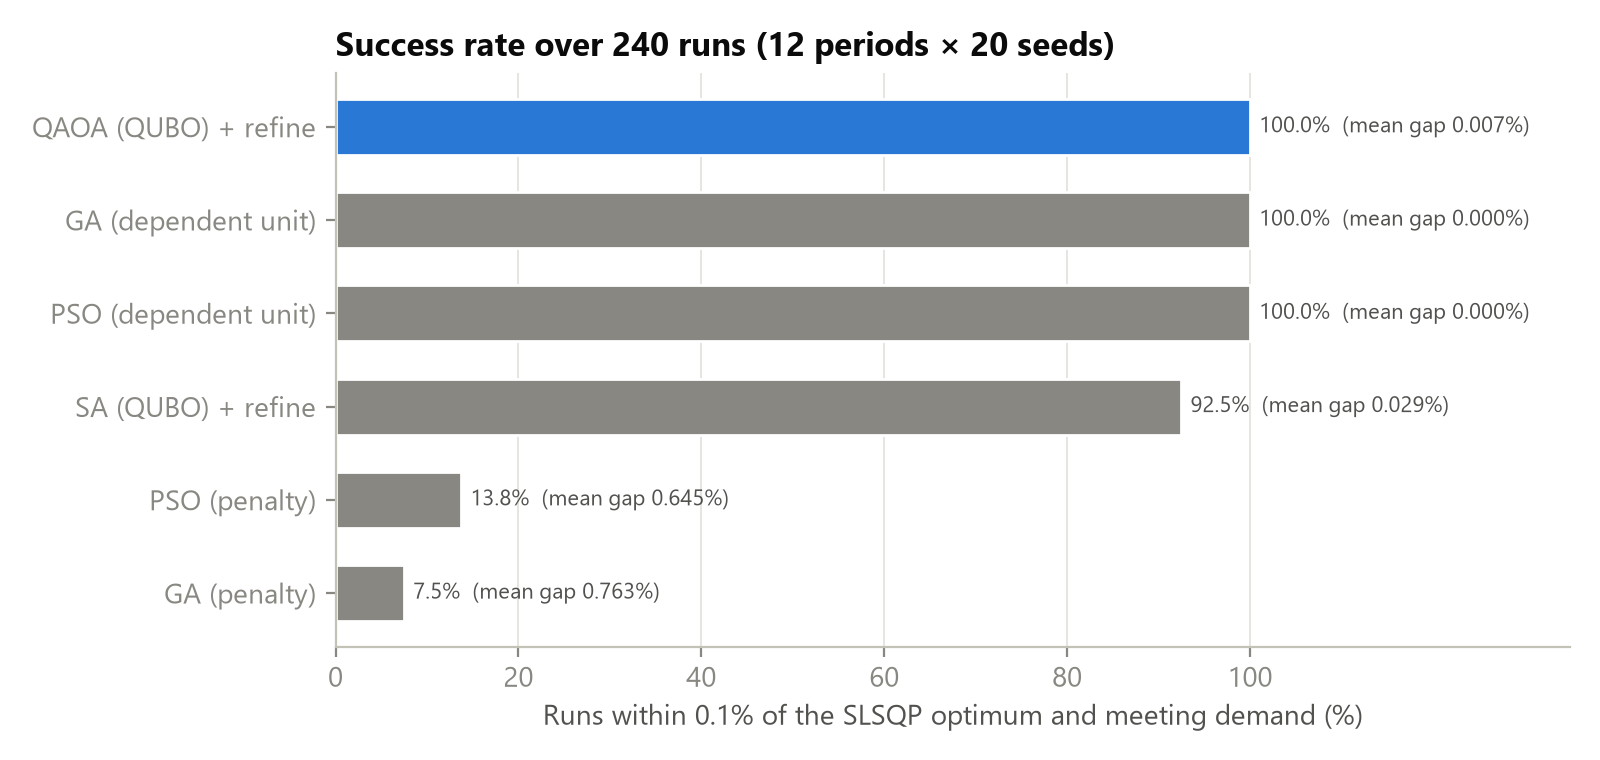
\includegraphics[width=0.9\textwidth]{baselines_success}
\caption{Success rate of the stochastic methods over 240 runs.}
\label{fig:baselines}
\end{figure}

The comparison shows the following.
\begin{itemize}
\item \textbf{Against the same binary problem}, QAOA performed as well as exhaustive search in every one of the 240 runs, with identical costs. Simulated annealing with the same budget and the same refinement succeeded in 92.5\,\% of runs, with a worst gap of 0.44\,\%. On this problem QAOA's sampling was therefore more reliable than SA.
\item \textbf{The 0.007\,\% mean gap of QAOA is a property of the 4-bit grid}, not of QAOA: exhaustive search, which by definition finds the QUBO optimum, gives the same value.
\item \textbf{Continuous heuristics} reach the exact optimum when the balance constraint is handled by the dependent-unit method of Gaing \cite{gaing2003}, because they are not limited to a grid. With a plain penalty they often stop at a nearby but more expensive dispatch (13.8\,\% and 7.5\,\% success). This shows that constraint handling matters as much as the choice of algorithm.
\item \textbf{Speed:} every classical method is faster than simulated QAOA. Simulating a quantum circuit on a classical computer costs time that grows exponentially with the number of qubits, so no runtime advantage can be expected here.
\end{itemize}


\section{Execution on IBM quantum hardware}
Table~\ref{tab:hw} and Figure~\ref{fig:hw} report the hardware experiment on \texttt{ibm\_marrakesh}, a 156-qubit IBM Heron processor (job \texttt{dc299oanj2vs73dgbsd0}, period 1, $p = 1$, 4096 shots).

\begin{table}[H]
\centering
\caption{IBM hardware results, period 1 (250 MW).}
\label{tab:hw}
\begin{tabular}{p{0.42\textwidth}cc}
\toprule
 & 6 qubits (2 bits/unit) & 9 qubits (3 bits/unit)\\
\midrule
Transpiled depth / two-qubit gates & 124 / 46 & 271 / 144\\
P(optimal): random / HW / sim. & 1.56 / 3.69 / 4.11\,\% & 0.20 / 0.24 / 0.53\,\%\\
P(near-opt.): random / HW / sim. & 12.5 / 18.9 / 24.2\,\% & 6.1 / 15.5 / 18.0\,\%\\
QUBO optimum measured on hardware & yes & yes\\
Hybrid cost gap & 0.000\,\% & 0.254\,\%\\
\bottomrule
\end{tabular}
\end{table}

\begin{figure}[H]
\centering
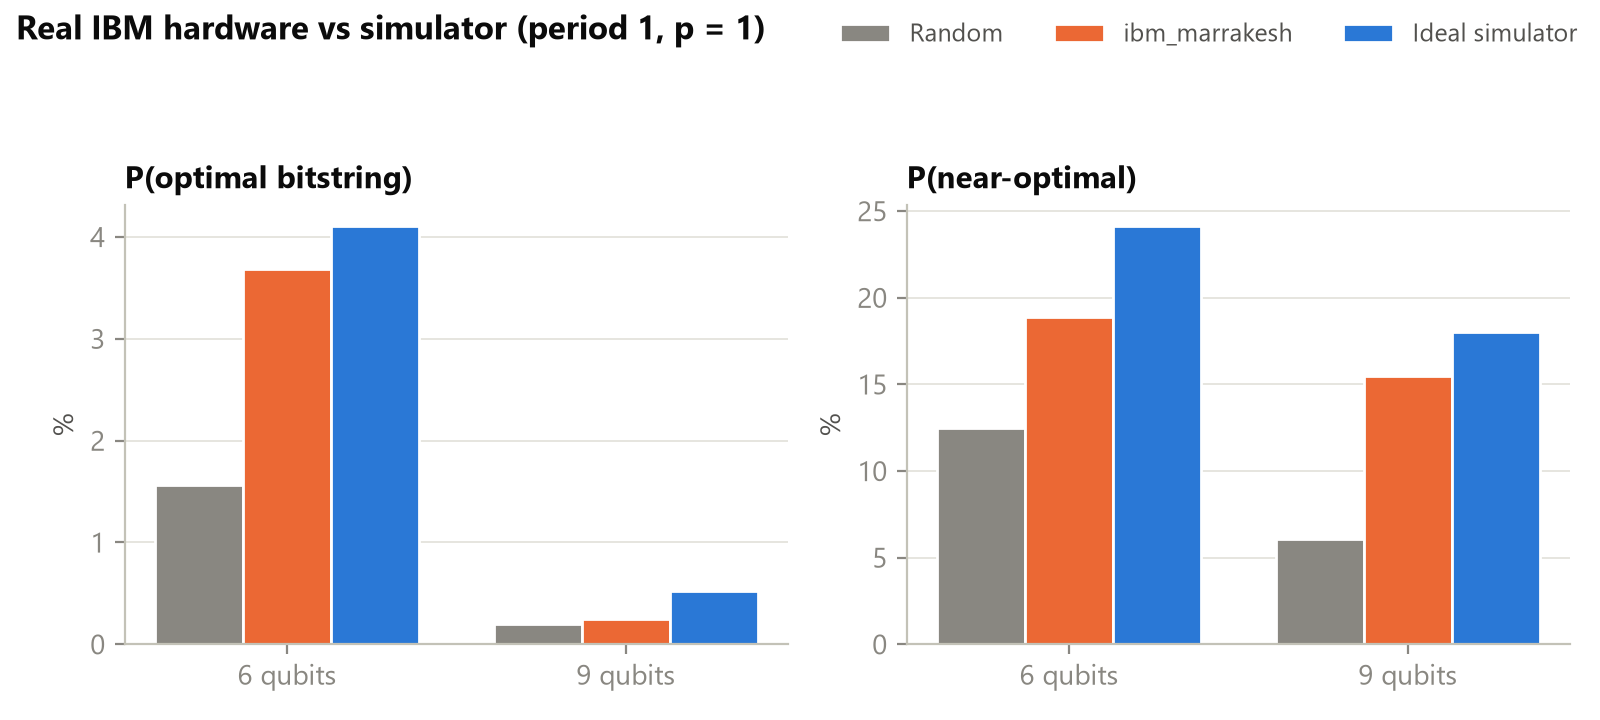
\includegraphics[width=0.9\textwidth]{ibm_hardware}
\caption{Real hardware against the ideal simulator and random sampling.}
\label{fig:hw}
\end{figure}

With 6 qubits, the hardware found the optimal bitstring 2.4 times more often than random sampling and kept about 90\,\% of the ideal simulator's probability; the refined dispatch equals the SLSQP optimum. With 9 qubits, the transpiled circuit needs 144 two-qubit gates, and gate noise reduces the gain on the optimal bitstring to 1.2 times random, although the near-optimal probability (15.5\,\% against 6.1\,\%) still shows a clear signal. The 9-qubit hybrid gap of 0.254\,\% comes from the coarser 3-bit grid (steps of 16--21~MW). These results show that the method runs on present hardware, and that noise, not the formulation, limits the problem size.

\section{Discussion}
\begin{itemize}
\item \textbf{Accuracy.} Hybrid QAOA reaches the SLSQP optimum to within 0.04\,\% in every period; the small remaining gap is set by the binary grid and the refinement box, not by QAOA.
\item \textbf{Quantum effect.} The trained circuit makes the optimal dispatch up to 31 times more likely than random sampling, and the gain grows with depth.
\item \textbf{Speed.} QAOA is not faster. On a laptop the simulator needs about 22~s of training and 0.2~s of sampling per period, while SLSQP needs about 1~ms. For a 3-unit convex problem, classical methods remain the right tool. No quantum speed-up is claimed.
\item \textbf{Where QAOA could help.} The value of the QUBO route lies in problems that are binary by nature, such as unit commitment, where classical solvers face combinatorial growth.
\end{itemize}
